\subsubsection{Time schedule}

To be able to plan our time efficiently, we had to find out how much time we had at our disposal. Our way of doing this was to create a custom spreadsheet containing all the dates until the final deadline.
For each date a field for each group member was made wherein the available time span for that person was entered. This way it was easy for us to get an overview of when we all were available. This helped us a lot in planning our meetings.

Generally we decided that if three or more group-members were available, a meeting would be planned. We would rather plan too many meetings and be done with everything early, than plan the exact hours needed to complete all the backlog items and risk time pressure due to unforeseen tasks or delays.

Through the use of the above method we avoided available time to be wasted as it had been during the first month of preparations. By planning all work to be done during meetings, we believed it would help all meeting participants to stay focused on their tasks, preventing the behavior we had experienced during the Easter holidays.

From the first part of the project we had learned that all-nighters - that is, a meeting continuing until the next morning - were effective ways to get a lot of work done, even though the productivity decreased over night. With this experience we converted as many pairs of subsequent days into all-nighters as we deemed it possible (see figure \ref{time_schedule}).

\begin{figure}[H]
  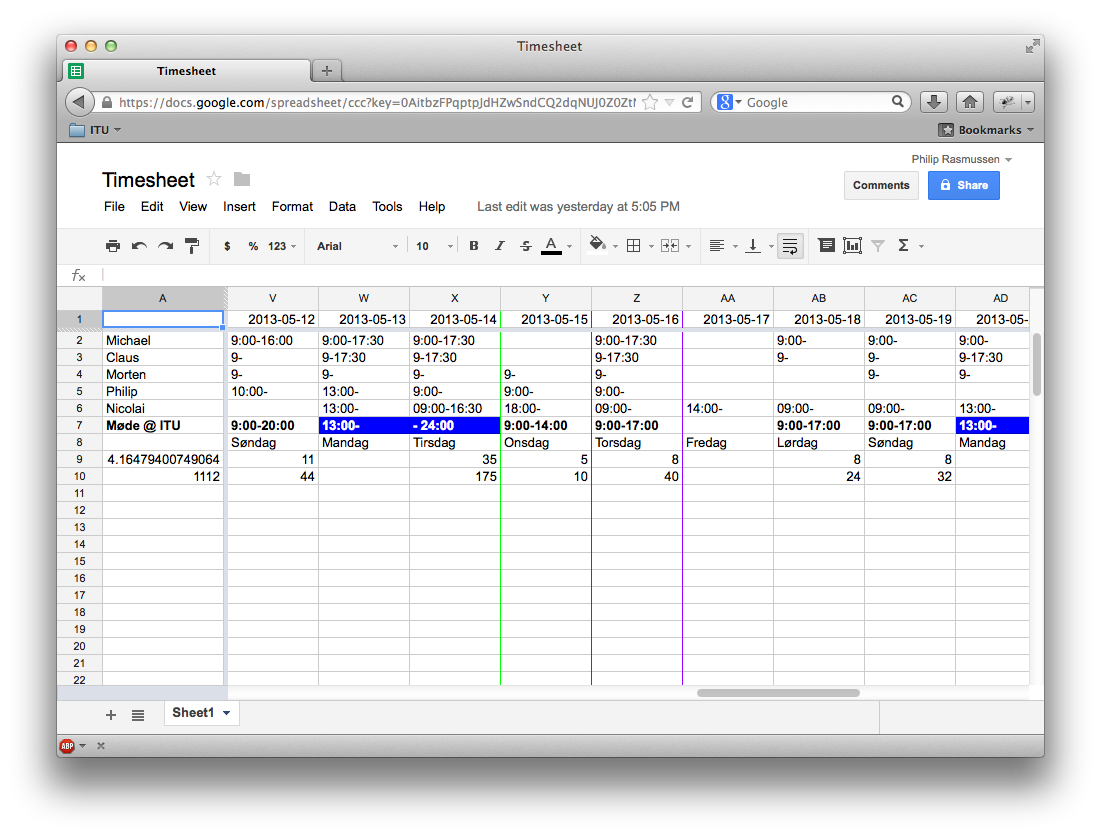
\includegraphics[width=\textwidth]{illustrations/partialTimeSheet}
  \caption{The time spreadsheet resulting from applying our custom method. The dates with bold time spans indicate days with meetings. The double fields with blue background indicate planned all-nighters. The colored, vertical lines indicate deadlines.}
  \label{time_schedule}
\end{figure}

We had great benefit from applying the method, as planning group meetings was instantaneous without too much discussion back and forth. At the time of writing, almost all meetings have been held as planned, although the all-nighters up to deadlines have been pushed a day for maximum efficiency with report writing.